\section{Final test and lesions on fresh missions}\label{sec:stageg}
All parts of this stage were written down with their thresholds before the runs (stage G). The test places are the same held-out
Tokyo and Kazan districts, but the 300 missions are new: new layouts, new texts, new rough points, new failures. Nothing in the
system was tuned on them.

\paragraph{The final test (G2).} Table~\ref{tab:g2} gives the system alone (the operator's text parsed by the F3b parser, no person
to answer questions) and the same system with the classic reflex in place of the feeling core, on the same 300 missions.
The main result of the project repeats on this fresh set and is larger than before: without the core, 14.7\,\% of missions touch the
static world, with it 4.3\,\% (paired difference $-10.3$ percentage points\ci{-14.7}{-6.0}; $-0.61$\ci{-0.92}{-0.35} contacts per
mission). For the first time the core also reduces hits by attacking birds ($-0.19$\ci{-0.33}{-0.06} per attacked mission), and
the system with the core completes more steps ($+0.038$\ci{0.008}{0.070}). The pre-registered safety rule was not met: the drone
alone touched a wrong target in 3 of 300 missions, 1.0\,\% with a bootstrap upper bound of 2.3\,\% (exact Clopper--Pearson bound 2.9\,\%) against the required 2\,\%. Fig.~\ref{fig:lesion}
puts this replication next to the first lesion study.

\begin{table}[t]
\centering\small
\caption{Final test on 300 fresh missions in unseen places (G2). Same missions for both variants; brackets are 95\,\% bootstrap
intervals over missions. The difference column is paired.}
\label{tab:g2}
\setlength{\tabcolsep}{3.5pt}
\begin{tabular}{@{}lccc@{}}
\toprule
 & Feeling core (alone) & Classic reflex & Difference \\
\midrule
Missions with a static contact & \textbf{4.3\,\%}\ci{2.3}{6.7} & 14.7\,\%\ci{10.7}{18.7} & $-10.3$\ci{-14.7}{-6.0}\,pp \\
Static contacts per mission & & & $-0.61$\ci{-0.92}{-0.35} \\
Attack hits per attacked mission & & & $-0.19$\ci{-0.33}{-0.06} \\
Steps done & 0.301\ci{0.254}{0.348} & 0.257\ci{0.214}{0.304} & $+0.038$\ci{0.008}{0.070} \\
Whole missions done & 0.287\ci{0.233}{0.340} & 0.253\ci{0.207}{0.303} & $+0.033$\ci{0.003}{0.063} \\
Wrong target (rule $\le 2$\,\%) & 1.0\,\%\ci{0}{2.3} & 2.3\,\%\ci{0.7}{4.0} & $-1.3$\ci{-3.0}{-0.3}\,pp \\
\bottomrule
\end{tabular}
\end{table}

\begin{figure}[t]
\centering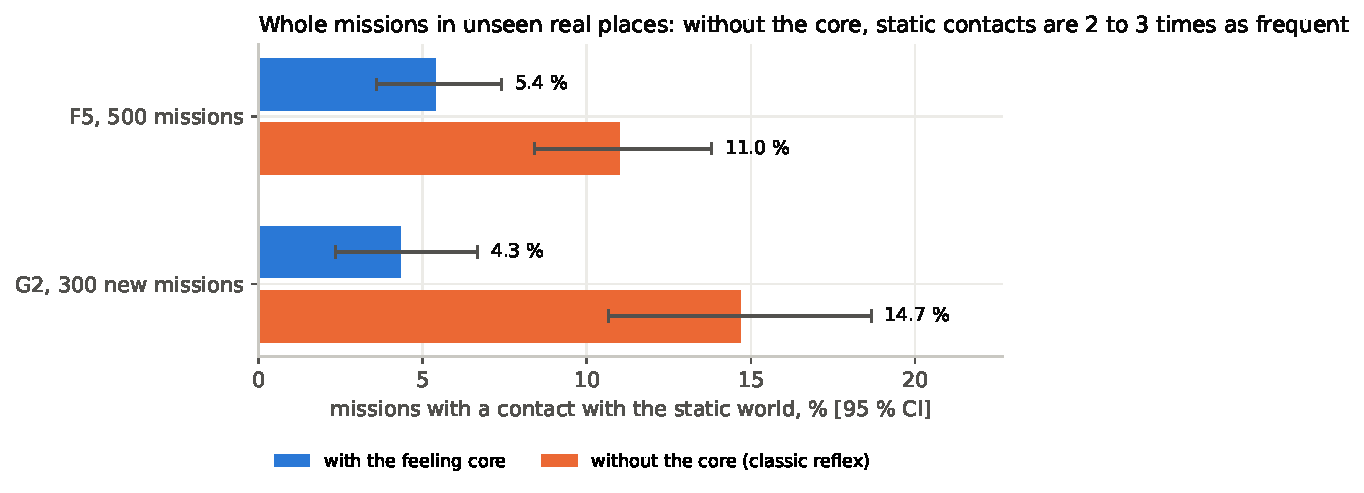
\includegraphics[width=.92\linewidth]{fig_missions_lesion.pdf}
\caption{Whole missions in unseen real places, with the feeling core and with a classic reflex in its place. F5: the first lesion
study (500 missions); G2: 300 fresh missions. Intervals: 95\,\% bootstrap over missions.}
\label{fig:lesion}
\end{figure}

\paragraph{Alone and with an operator.} By action, the drone alone completed fly-by in 0.49 of steps, landing 0.44, inspection 0.30,
hook pick-up 0.29, parachute drop 0.22 and hangar entry 0.14. Most failures are refusals by design: when the description
does not single out one object, the drone does not touch any. The app is meant to be used with a person who checks the parse and
answers the drone's questions, so we flew the first 200 missions once more that way. The simulated operator gets the true parse
and, when asked, picks the candidate view that lies at the meant object. On the 182 missions that finished within the run's time
limit (18 were still flying), the drone with an operator completed 0.56 of steps against 0.29 alone on the same missions (paired
$+0.27$\ci{0.20}{0.33}) and 0.54 of whole missions against 0.29 (Fig.~\ref{fig:actions}). Most missions needed no question at all
(median 0, 90th percentile 1). The help has a cost: the drone now flies every step to the end, and missions with a static contact
rose from 3.8 to 10.4\,\% ($+6.6$\ci{2.7}{10.4} points). It touched a wrong target in 4 missions (2.2\,\%); two of them are the
same mistakes it made alone, without asking. In three missions, when none of its candidates was the target, the drone asked again
and again (131 to 541 times): the app needs a limit there.

\begin{figure}[t]
\centering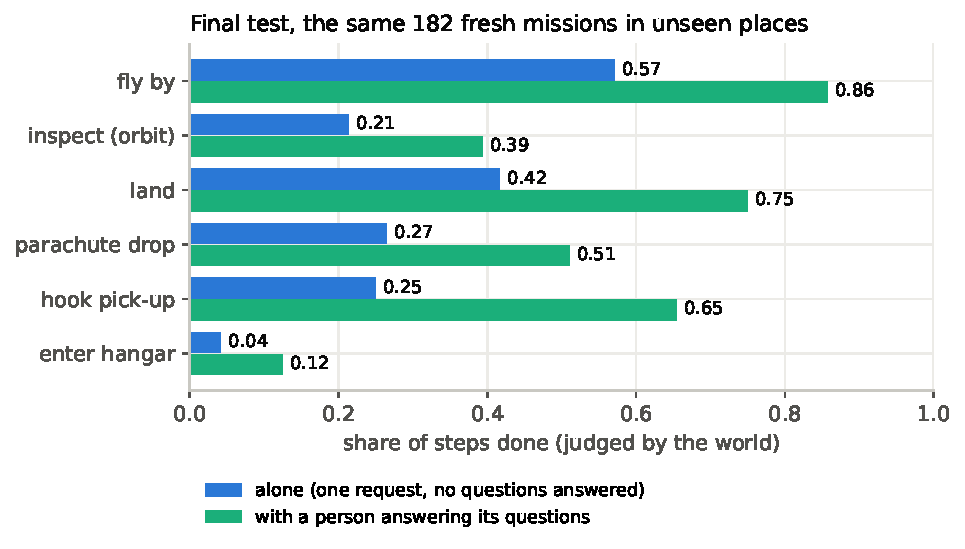
\includegraphics[width=.8\linewidth]{fig_actions.pdf}
\caption{Steps done by action on the same 182 fresh missions, by the drone alone and with a person who checks the parse and answers
its questions. Judged by the world: what it landed on, where the parcel fell, what hangs on the hook.}
\label{fig:actions}
\end{figure}

\paragraph{The hangar door (G1).} Hangar entry was the weakest action, and one traced failure showed the door finder taking a gap
in the back wall for the door. We tried a stricter rule: an opening counts only if the lidar sees the hangar's floor through it.
With the drone placed on the circle around 90 hangars, the old finder found the right door of 74 of 76 open hangars and no door in
any of 14 closed ones; the new one found 72, missed 4, and saw a door in 3 closed hangars. In flight, with the true parse and a
person answering the drone's questions, the new finder entered 1 hangar in 38 flights and the old one 6 in 37: the drone's own
position drifts while it circles, and the drift smears wall points across the box. By the rule written beforehand the old finder
stays.

\paragraph{Slow feelings in hard missions (G3).} The slow feelings (``I am lost'', ``low energy'') hardly ever fired in the short
missions of F5, so stage G tested them where they should matter. The 120 hard missions in the test places start with 30--65\,\%
charge, have a cold battery in 60\,\% of missions, wind of 3--9\,m/s, a lost GPS (47 of the 99 missions flown) or a spoofed one (26), bird attacks, and always require
the return home. The parse is true, so only the slow layer is tested. Five variants flew the same missions: the core's feelings;
raw telemetry with thresholds instead, which compares the charge with the energy needed to fly home; no slow layer; and each
feeling removed in turn. The time cut left 99 missions (98 for three variants; Fig.~\ref{fig:slow}).

With the core's feelings the battery died in the air in 29\,\% of missions, and without any slow layer also in 29\,\% (paired
difference $0.0$\ci{-7.1}{7.1} points). The first expectation, that the slow layer prevents such falls, is not confirmed. Raw
telemetry did better: 16\,\% falls ($-13.1$\ci{-21.2}{-5.1} points against the feelings) and more landings at home (63 against
52\,\%, $+11.1$\ci{5.1}{18.2}). It paid with fewer whole missions ($-0.040$\ci{-0.081}{-0.010}) because it turned home early twice
as often. H6 is therefore not confirmed, as we had written down beforehand: the ``low energy'' feeling was trained on 40-s
episodes and does not know the distance home, while the telemetry rule multiplies the drain by that distance. The feeling did act
(with it the drone turned home early in 13\,\% of missions, without it never), but the falls did not change ($0.0$\ci{-6.1}{6.1}).
Removing ``I am lost'' changed neither falls nor returns. One observation was not planned: without ``I am lost'' the drone touched
the static world less ($-0.22$\ci{-0.43}{-0.06} contacts per mission). For a real aircraft the lesson is plain. The energy reserve
must come from an explicit rule over distance and drain, not from a learned feeling.

\begin{figure}[t]
\centering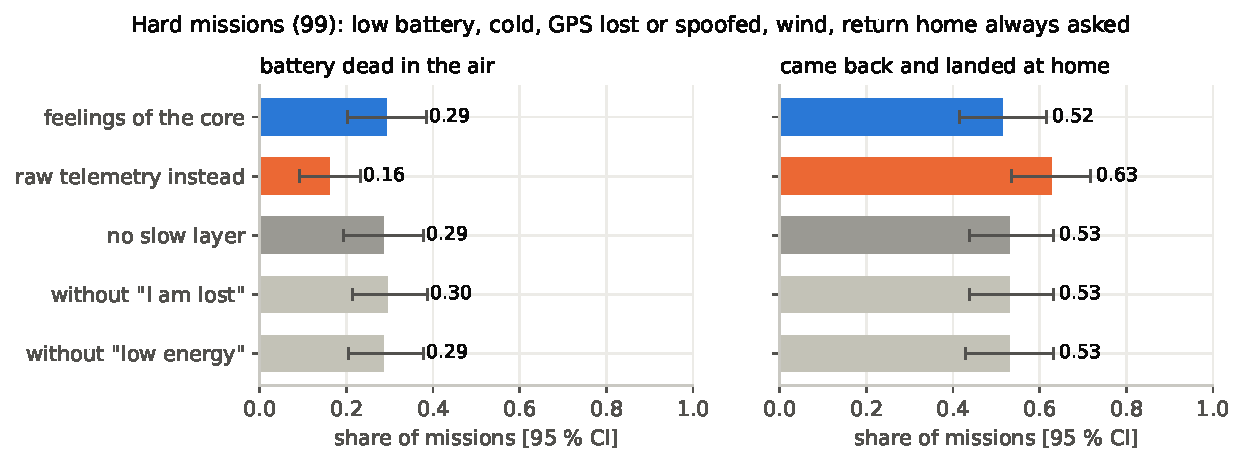
\includegraphics[width=\linewidth]{fig_slow.pdf}
\caption{Hard missions (G3), the same missions for all variants. Left: missions in which the battery died in the air. Right:
missions that ended with a landing at home. Raw telemetry with an energy-to-home rule beats the learned slow feelings; removing
the slow layer or a single feeling changes nothing. Intervals: 95\,\% bootstrap over missions.}
\label{fig:slow}
\end{figure}

\paragraph{False and delayed feelings (G4).} Damasio's patients suggest two more lesions: a feeling that fires when nothing is
there, and one that comes too late. On the first 100 missions of the final test we flew the full system twice more. In the first
variant the ``keep going'' marker reported danger in an empty sky for 1\,s at random moments, about once every 20\,s; in the
second the markers saw the world 0.3\,s late. False alarms added 24 overrides per mission\ci{19}{29} and did not cost steps
($+0.015$\ci{-0.05}{0.08}), but missions with a static contact rose from 4 to 9\,\% ($+5.0$\ci{0.0}{10.0} points): a needless
swerve in a street can itself end in a wall. We had expected fewer steps and no fewer contacts; the second half held, the first did
not. A 0.3-s delay changed little: missions with a static contact $+3.0$\ci{-1.0}{8.1} points, so the expected rise is not
confirmed. The markers look 2\,s ahead, and a 0.3-s lag is small against that horizon.

\subsection{Towards a real aircraft: the brain on the PX4 flight stack}\label{sec:px4}
A drone flies on an autopilot, not on our simulator's controller. We wrote a MAVLink bridge that gives the unchanged mission brain
the same interface on a real autopilot (PX4 \citep{meier2015px4} or ArduPilot): telemetry in, velocity set-points out at 20\,Hz, frame conversions, a
watchdog that holds position when the brain is slow, and the autopilot's own failsafes underneath. We then flew 12 missions
(landing, drop, pick-up, inspection, fly-by, ground-level targets) with PX4's software-in-the-loop build and its SIH quadrotor
model, posing our world at PX4's estimated pose every 0.1\,s so that the lidar, the camera and the scoring stay ours. The bridge
worked mechanically: PX4 armed, took off, flew the brain's commands, landed, re-armed and refused to arm when its simulated
sensors failed. Mission success did not transfer: 1 of 12 missions with PX4 against 7 of 12 with our controller on the same
missions, and holding position through PX4's own position loop in the precise phases did not change the count. PX4 tracks the
brain's velocity commands with a median error of 0.8--1.3\,m/s and missions took about twice as long. The brain's timeouts, speeds and
precision phases were tuned on our controller; they must be re-tuned and re-tested on the real flight stack before any flight.
